\begin{figure*}[t!]
    \centering
    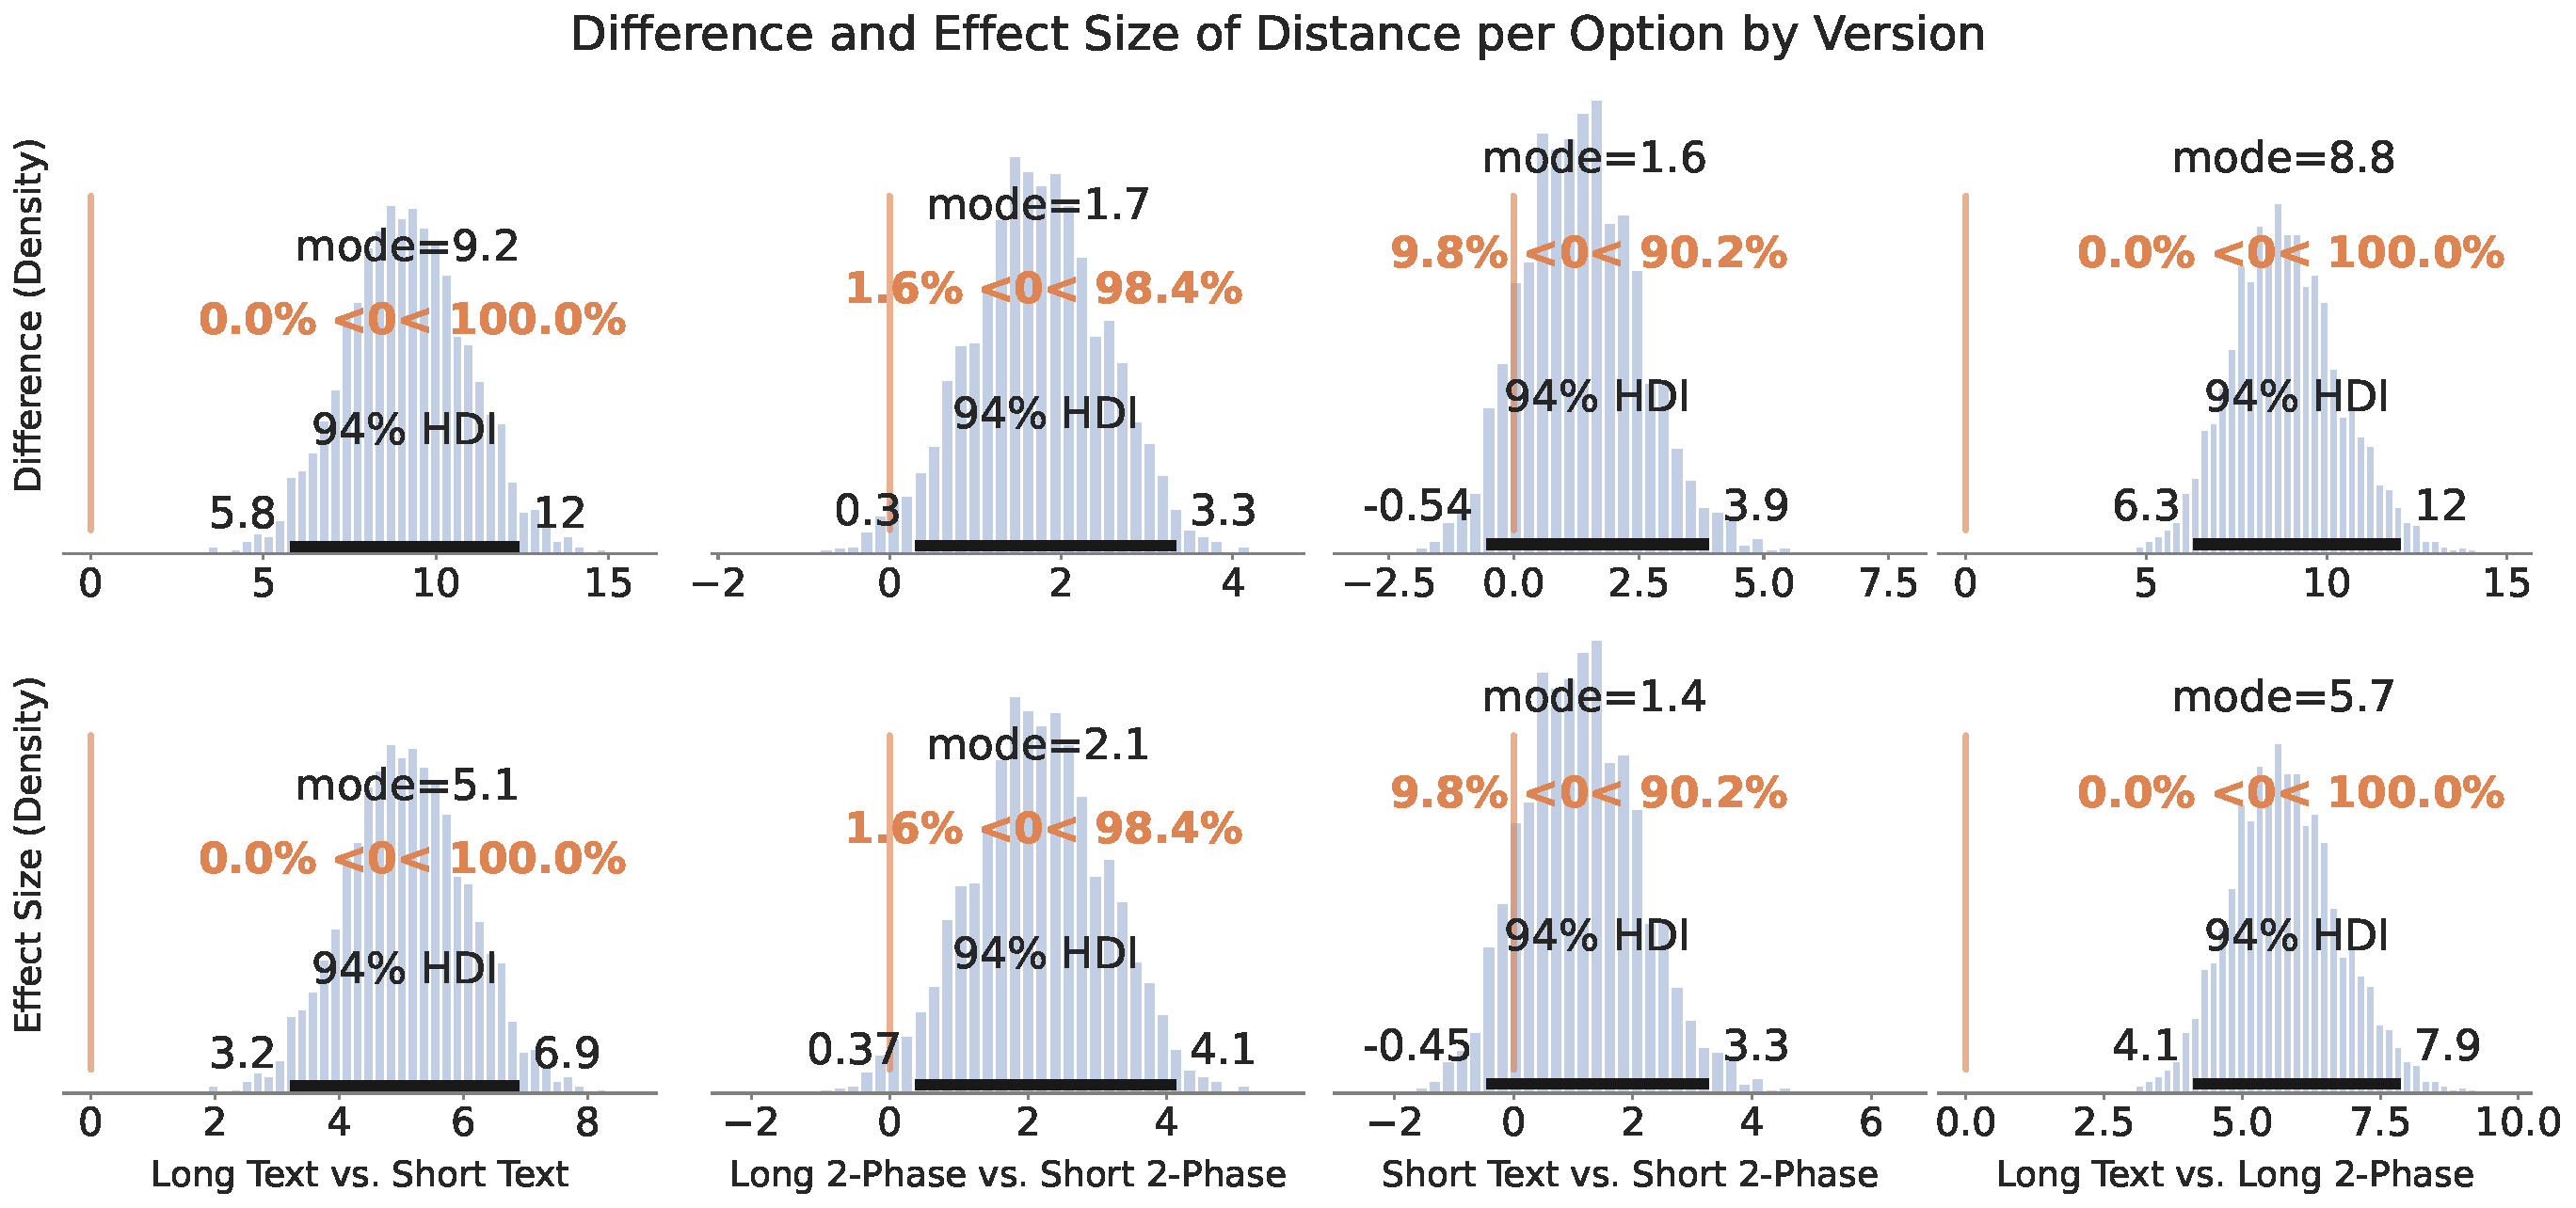
\includegraphics[width=0.75\textwidth]{content/image/distance/distance_diff_per_option_effect_size_by_version.pdf}
    \caption{The figure shows the contrast distributions of the mean edit distance per option between pairwise experimental conditions, with the first row representing absolute differences and the second row depicting effect sizes.~\textbf{Main takeaway:} is that participants in the long text estimated more edit distance per option compared to those in the short text and the long two-phase condition. Notably, the long two-phase interface required estimated only slightly more edit distances despite the longer survey length.}
    \Description{A grid of histograms titled "Difference and Effect Size of Distance per Option by Version," showing posterior distributions for differences (top row) and effect sizes (bottom row) across four experimental comparisons. Each plot includes density (y-axis) against either difference or effect size (x-axis). Key values are annotated in orange above each histogram. The vertical line at zero serves as a reference point for interpreting the directionality of the differences and effect sizes. In this plot, the orange line lies outside of the ROPE for differences between long and short text; long 2-phase and short 2-phase; and long text and long 2 phase, signifying statistical differences among these comparisons.}
    \label{fig:dist_per_option_bayesian}
\end{figure*}

\section{Clickstream data: Interface reduces edit distance in long surveys}
\label{sec:dist}
Following our findings on cognitive load, we analyze voting behaviors to identify differences in how participants cope with survey lengths, how interfaces influence their behavior, and why the long text interface might exhibit lower cognitive load. All data are publicly available\footnote{https://github.com/CrowdDynamicsLab/Quadratic-Survey-Dataset-and-Analysis} to ensure transparency and support further research. This measure reveals how participants navigate and engage with survey options. We examine three dimensions of this measure: edit distance per option, edit distance per action, and cumulative edit distance throughout the survey.

\begin{figure}[h!]
    \centering
    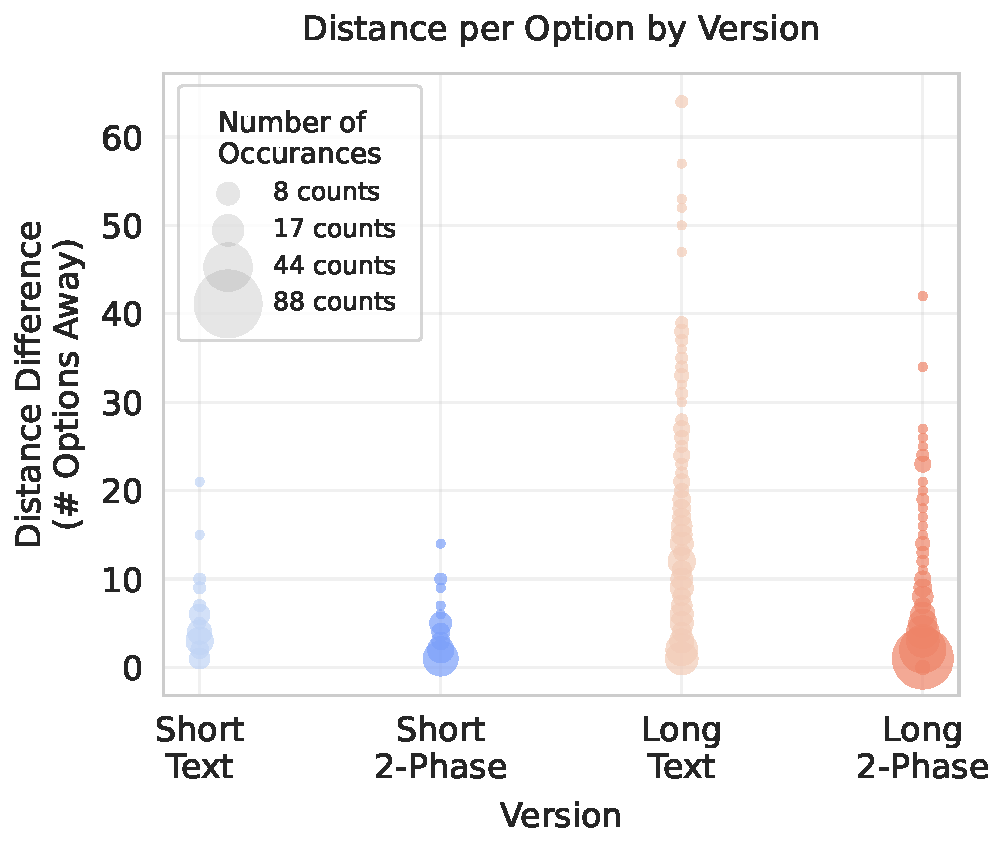
\includegraphics[width=0.47\textwidth]{content/image/distance/distance_diff_by_version.pdf}
    \caption{Edit Distance Per Option: We sum the total number of edit distances for each option, with the figure using the radius to indicate how often a specific edit distance occurred within an experimental condition.~\textbf{Main takeaway:} Participants in the two-phase interface completed their votes for more options with fewer edit distances, whereas the Long Text interface shows a long tail of options requiring a wider range of edit distances.}
    % \vspace{-10pt}
    \Description{A bubble plot titled "Distance per Option by Version" showing the distribution of distance differences (y-axis, measured as the number of options away) across four experimental versions (x-axis): Short Text, Short 2-Phase, Long Text, and Long 2-Phase. The size of the bubbles range from 8 counts (smallest bubble) to 88 counts (largest bubble). Trends: The largest bubbles (highest frequency) occur closer to zero distance difference, particularly in Short Text and Short 2-Phase. Higher distance differences appear more frequent in the Long Text and Long 2-Phase conditions. The visualization emphasizes the variability and frequency of distance differences for each version, with bubble size providing a visual cue for occurrences.}
    \label{fig:dist_per_option}
\end{figure}

\begin{figure*}[h!]
    \centering
    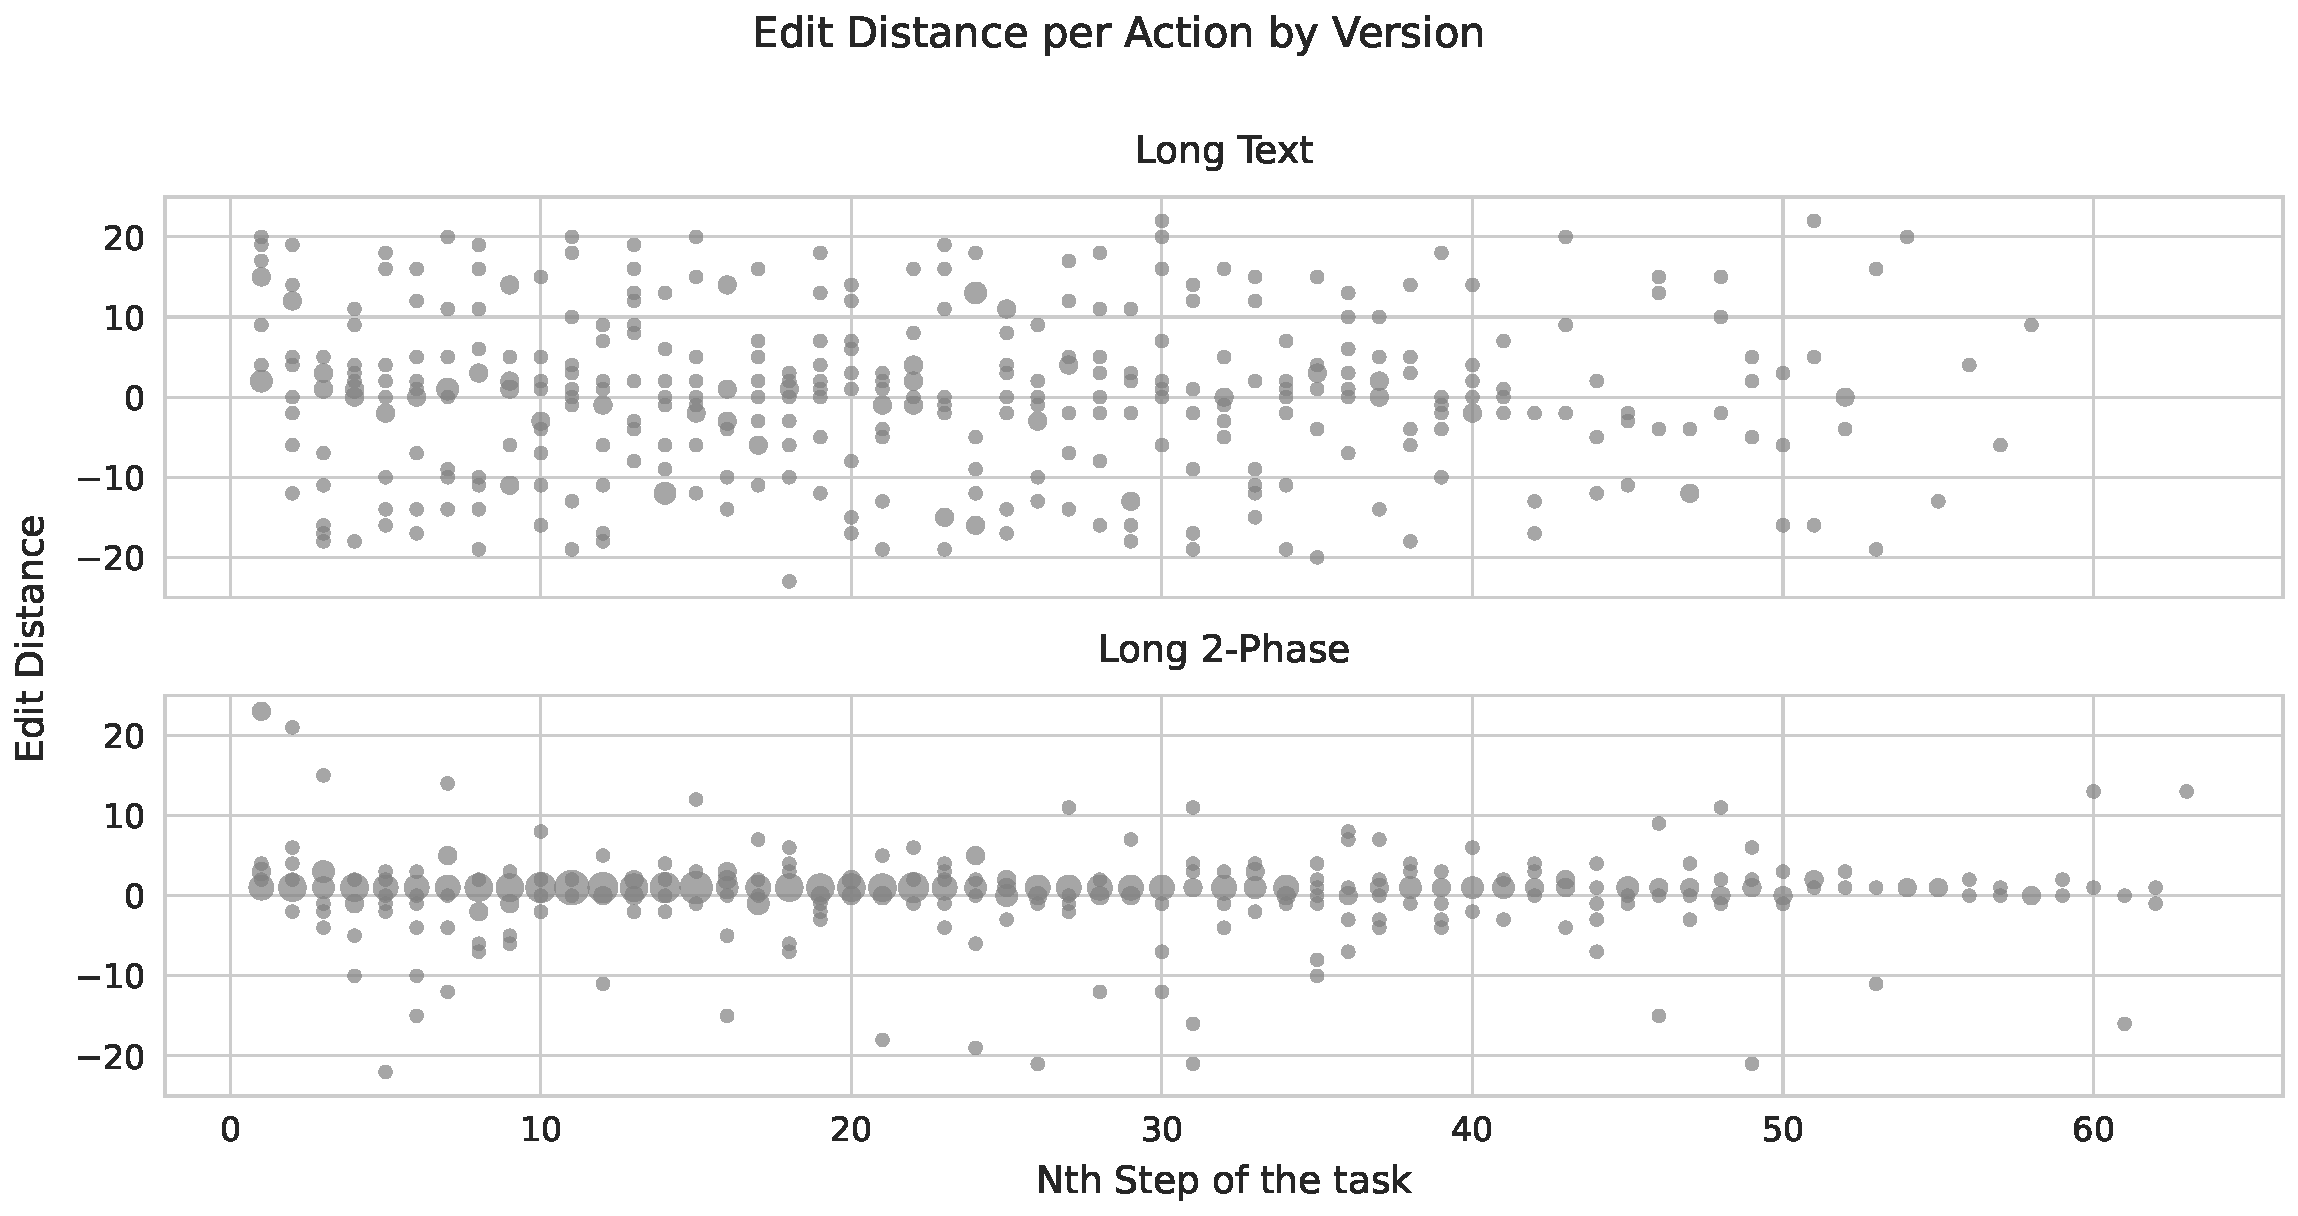
\includegraphics[width=0.75\textwidth]{content/image/distance/edit_distance_per_action_by_version.pdf}
    \caption{Edit Distance Per Action: This plot shows the frequency of specific edit distances at each step across the text interface and two-phase interface.~\textbf{Main takeaway:} Participants in the long two-phase interface tend to make adjustments closer to their previous actions, resulting in visually less variance in edit distances throughout the entire survey.}
    \Description{A two-panel scatter plot titled "Edit Distance per Action by Version," comparing edit distances across task steps for two conditions: Long Text (top panel) and Long 2-Phase (bottom panel). The Y-Axis represents the Edit Distance, ranging from -20 to 20, representing the magnitude of deviations in task execution. the X-Axis: Nth Step of the Task contains values increasing up to 60, indicating progression through task steps. Top Panel (Long Text): Shows a dispersed pattern of points with no clear trend, indicating variability in edit distances throughout the task steps. Bottom Panel (Long 2-Phase): Displays a more compressed spread of points closer to zero, suggesting reduced variability in edit distances compared to the Long Text condition. The scatter plot highlights differences in task execution consistency between the two versions, with denser clusters near zero indicating closer adherence to expected task paths.}
    \label{fig:step-over-distance}
\end{figure*}

\textbf{Edit distance per option:} We calculate the total number of options a participant traversed when adjusting votes for a single option. Figure~\ref{fig:dist_per_option} illustrates differences across experimental conditions, with the long text interface showing the largest variance in the distance traveled and the highest mean. We implement a hierarchical Bayesian framework to model edit distance differences across experimental conditions. The observed distance differences are modeled using an exponential distribution, where the scale parameter is linked to survey length (treated as an ordinal variable), interface type (treated as a categorical variable), interaction effects between length and interface, and controlling for individual user variability. The linear predictor includes a global intercept and slope for length, random effects for each interface condition with an LKJ prior that captures the correlations among interface categories, and user-specific random effects to account for individual heterogeneity. Appendix~\ref{sec:apdx:model_distance_option} includes the detailed model.

Figure~\ref{fig:dist_per_option_bayesian} illustrates the pairwise posterior distributions for differences in edit distances across experimental conditions. For example, the difference in edit distances between the short and long static interfaces has a mode of 9.1, with a 94\% highest density interval (HDI) of [6, 13]. This indicates that participants in the long text interface move approximately 9.1 steps more than those in the short text interface, with a high degree of confidence. The effect size is large (mode = 5.1, 94\% HDI = [3.3, 7.1]), suggesting a statistically significant difference, which is expected due to the greater number of options in the long text interface.

Similarly, two-phase interface participants make approximately 8.9 fewer steps per option (mode = 8.9, 94\% HDI = [6.4, 12]) than those in the long text interface, with a large effect size (mode = 5.7, 94\% HDI = [4.2, 7.9]). The increase in edit distances between the short and long two-phase interfaces is substantially smaller (mode = 1.7, 94\% HDI = [-0.01, 3.1]) compared to their static counterparts. Comparing the short text and short two-phase interfaces shows limited difference (mode = 1.3, 94\% HDI = [-0.78, 3.8]), though the posterior distribution favors fewer steps for the two-phase interface (89.3\% probability). The model suggests that the two-phase interface reduces edit distance per option, particularly for the long QS.

\textbf{Edit distance per action:} Building on the statistical disparities observed in the previous analysis and the unique patterns exhibited by long text interface participants, we present analyses focusing on edit distance per action and cumulative edit distance throughout the survey between the long text and long two-phase interfaces. Edit distance per action measures how far participants move during each adjustment while completing the survey. Figure~\ref{fig:step-over-distance} illustrates how, at each step, the number of participants moving a given distance (represented by the size of the dots) varies across experimental conditions. Visually, participants move less on average per option within the two-phase interface, with lower variance at smaller scales. This indicates that participants are making local edits, meaning their adjustments tend to occur near their previous edits in terms of edit distance. This also highlights that the organization phase effectively adjusts option positions for easier access, despite participants still having the freedom to move across the interface as all options are presented to them.

In contrast to earlier analyses, we use a hierarchical Bayesian model (detailed in Appendix~\ref{sec:apdx:model_distance_variance}) to jointly estimate the mean and variance of edit distances across experimental conditions. The model assumes that edit distances are continuous and follow a normal distribution. This approach accounts for both central tendencies and variability, using separate predictors for the mean and variance. The model includes hierarchical effects for survey length, interface type, interactions between length and interface, and user-level random effects. Non-centered parametrization is used for survey length and interface type to improve convergence, while interaction effects are modeled with an LKJ prior to capture the correlations between factors. % User-level random effects reflected individual differences in behavior, incorporating variability into the model.

Figure~\ref{fig:step-over-distance_bayesian} illustrates the posterior variance distributions, confirming our hypothesis. Participants in the long text interface exhibit greater variance in movement, frequently navigating across the interface, compared to those in the long two-phase interface. This is evidenced by a variance difference mode of 76 (95\% HDI = [59, 99]) and a large effect size (mode = 7.1, 95\% HDI = [5.5, 9.2]).

\begin{figure}[ht!]
    \centering
    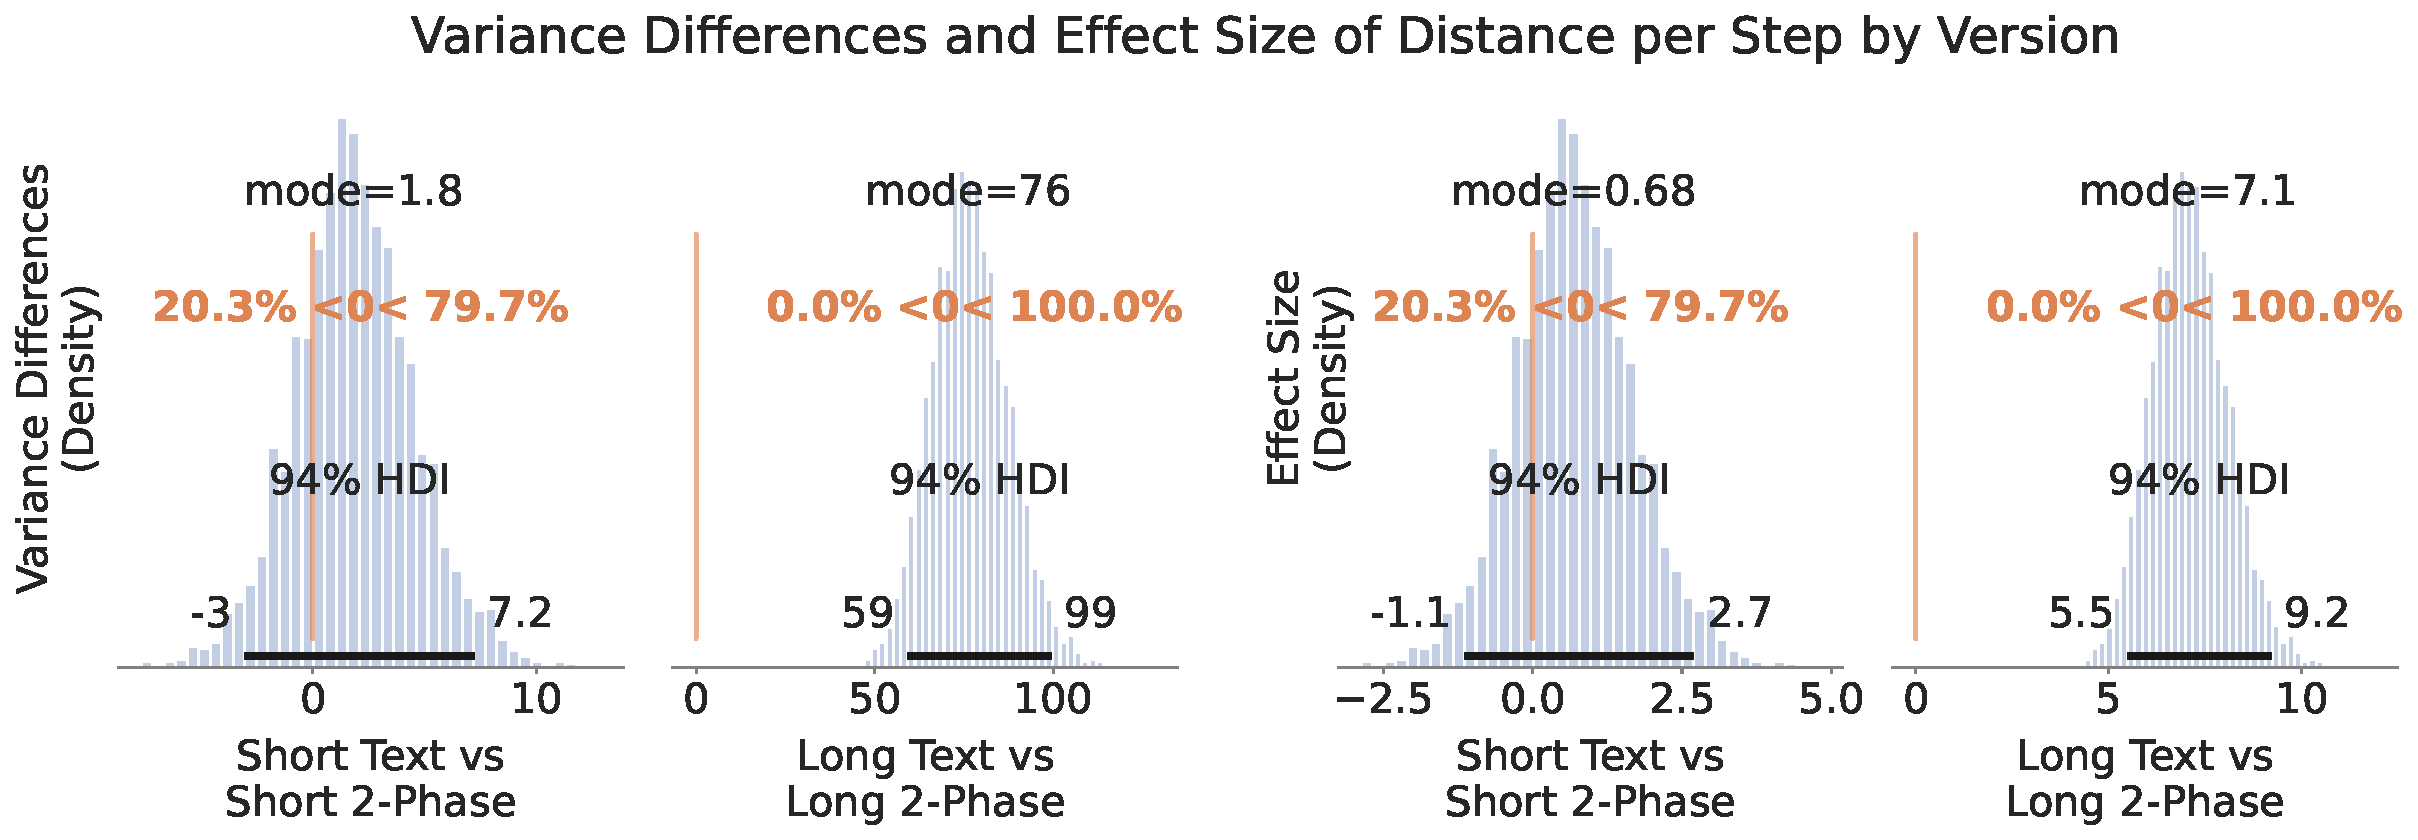
\includegraphics[width=0.4\textwidth]{content/image/distance/distance_diff_per_step_effect_size_by_version.pdf}
    \caption{The figure shows the contrast distributions of the mean edit distance per step between the two-phase interface and text interface for different survey lengths. The left two subplots represent absolute differences, while the right two depict effect sizes.~\textbf{Main takeaway:} long text participants exhibited greater variance in edit distance per step compared to those in the long two-phase interface. Similarly, the short text condition showed higher differences, although these were not statistically significant in Bayesian terms.}
    \label{fig:step-over-distance_bayesian}
    \Description{A grid of histograms titled "Variance Differences and Effect Size of Distance per Step by Version," displaying posterior distributions of variance differences (left) and effect sizes (right) for two experimental comparisons. Each plot includes density (y-axis) against variance differences or effect sizes (x-axis) with key statistics. Each histogram features annotated key values in orange and a vertical reference line at zero for interpretation. The distributions emphasize significant differences in variance and effect sizes across conditions, particularly for the Long Text vs. Long 2-Phase comparison, which shows consistently large and significant values.}
\end{figure}

\textbf{Cumulative edit distance for a participant:} Figure~\ref{fig:cumulative-distance} illustrates how the two-phase interface reduces per-action distance, accumulating over time. Some long text participants traverse double the amount of distance to complete the task compared to the long two-phase participants. We model this growth rate using a hierarchical Bayesian regression model (Detailed in Appendix~\ref{sec:apdx:model_cum_distance}), with cumulative distance as the predictive variable. The experimental variables include interface type as a categorical variable, individual users modeled with random effects, and steps taken as a continuous variable. A truncated normal likelihood constrains cumulative distances to positive values and varies these distances across steps for each participant while masking incomplete data.

Figure~\ref{fig:slope-diff-effect} shows that the slope for the long text interface is approximately 4.7, meaning each step by the text interface would add 4.7 edit distance (94\% HDI = [4.2, 5.4]), compared to the long two-phase interface, which shows a statistically significant difference with a mode of 1.4 (94\% HDI = [1.3, 1.7]). These results explain that the variance in edit distance per action and the increase in per option edit distance are consistent across participants between the two groups, showing that the organization phase allows participants to focus on adjusting options within proximity without having to navigate the interface to locate and make adjustments throughout the voting phase.

\textbf{Evidence from qualitative analysis:} Recall the differences in sources of cognitive load between the two experimental conditions: while two-phase interface participants make localized adjustments with nearby options, they experience cognitive demand from preference construction due to broader considerations that involve more options and higher-order values. Similarly, the qualitative results highlight that long text interface participants construct narrower preferences, yet their edit distance indicates broader movements across options.

Fewer long two-phase interface participants (60\%, N=6) reported precise resource allocation as a source of demand compared to 90\% in the text interface (N=9). We interpret this as former participants construct preliminary preferences during the organization phase, easing them to concentrate vote decisions as they focus more on deliberate preference building rather than mere completion. Conveniently positioning options with similar preferences reduced the need to look for an option and traverse the interface, allowing participants remain engaged in vote adjustments.

\begin{figure}[ht]
    \centering
    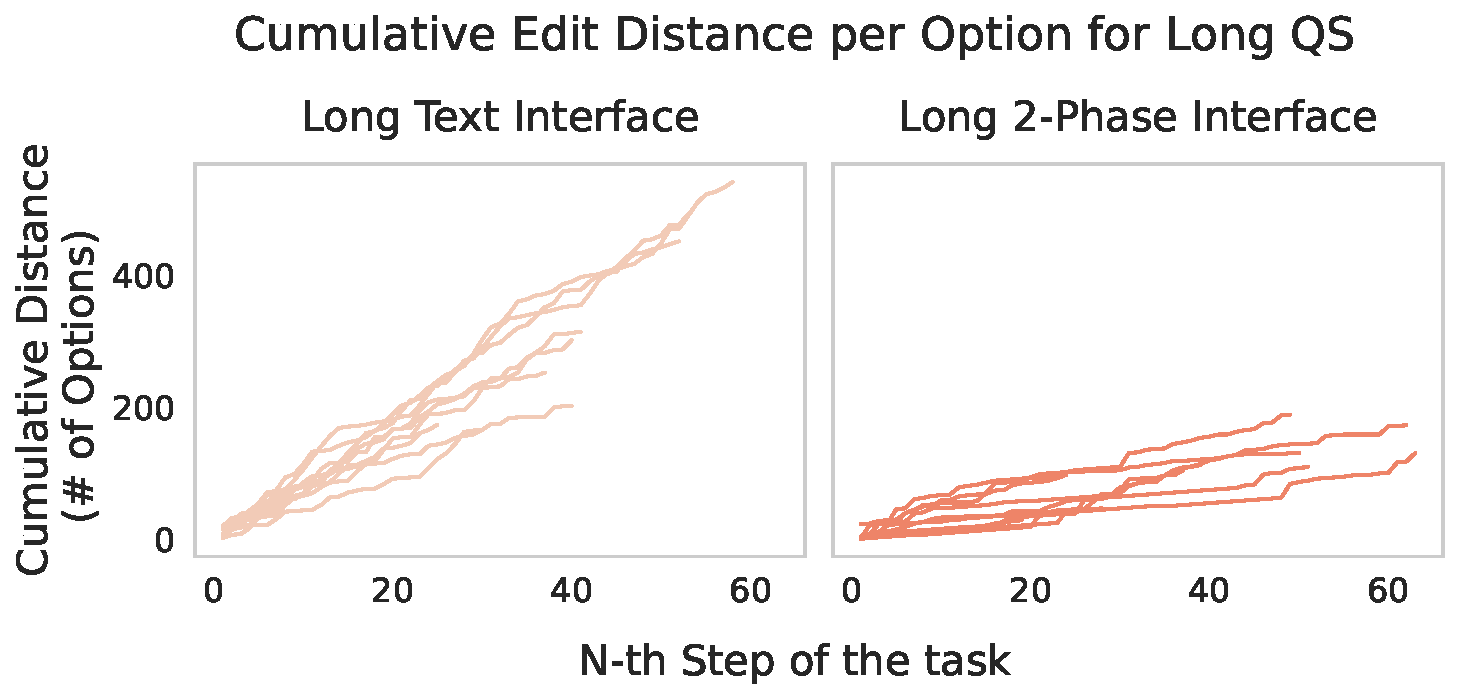
\includegraphics[width=0.47\textwidth]{content/image/distance/cumulative_edit_distance_per_option_long_qs_v3v4.pdf}
    \caption{This plot shows how the cumulative edit distances gained over the course of the survey between long text and long two-phase groups.~\textbf{Main takeaway:} Participants in the long two-phase interface tend to make smaller, more incremental adjustments, resulting in a visually flatter slope compared to the text interface.}
    \label{fig:cumulative-distance}
    \Description{A two-panel line plot titled "Cumulative Edit Distance per Option for Long QS," comparing cumulative edit distances across task steps for two conditions: Long Text (left panel) and Long 2-Phase (right panel). Y-Axis: Cumulative Distance (# of Options), ranging from 0 to 500, indicating the accumulated edit distances over task steps. X-Axis: Nth Step of the Task, ranging from 0 to 60, representing task progression. Left Panel (Long Text): Shows multiple trajectories of cumulative edit distances with a wider spread, reaching up to 500, indicating higher variability and more significant cumulative distances across task steps. Right Panel (Long 2-Phase): Displays tighter trajectories with cumulative distances reaching approximately 300, suggesting more consistent and lower cumulative edit distances compared to the Long Text condition. The plot highlights differences in task completion consistency and edit distance accumulation between the two conditions, with the Long 2-Phase condition demonstrating more controlled and efficient task execution.}
\end{figure}

\begin{figure}[ht]
    \centering
    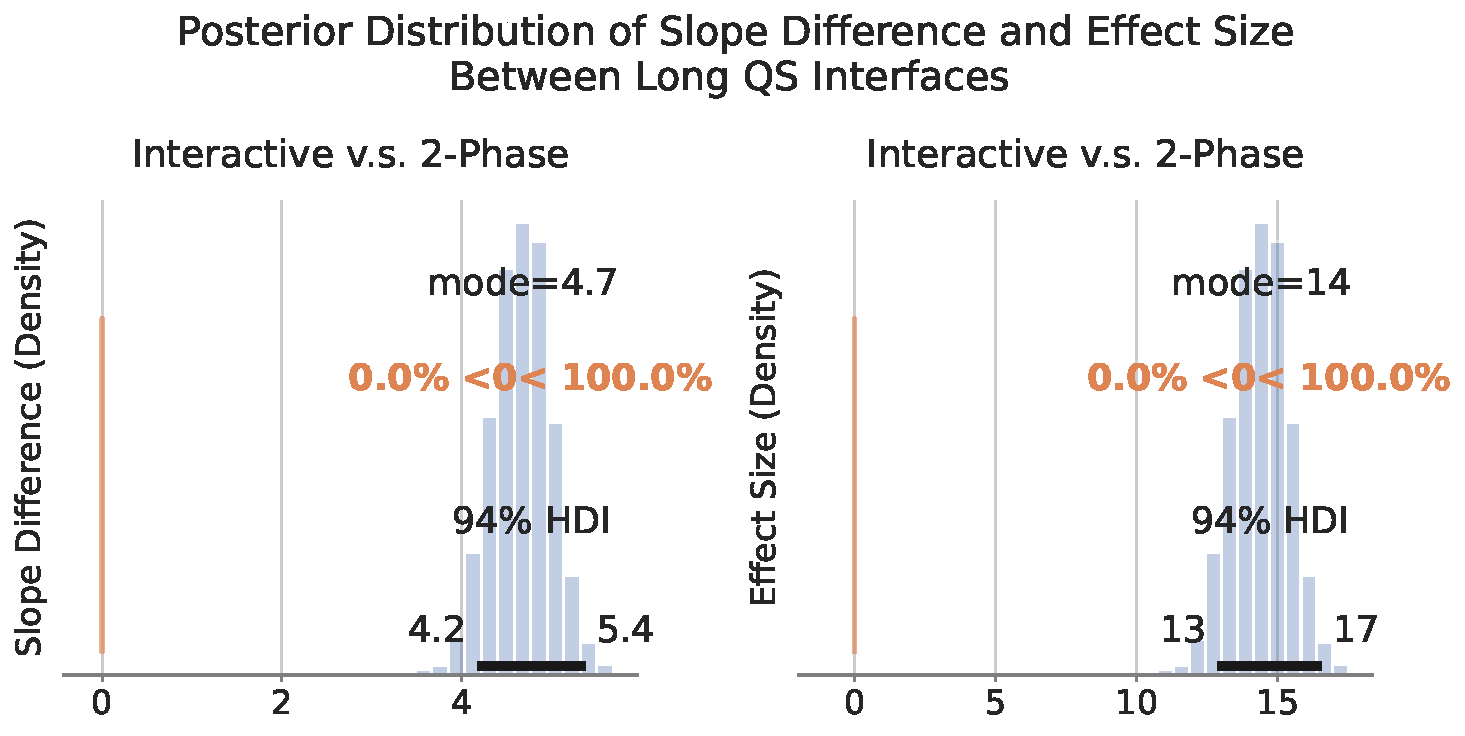
\includegraphics[width=0.47\textwidth]{content/image/distance/slope_diff_and_effect_size.pdf}
    \caption{The figure shows the contrast distributions of slope differences in cumulative edit distance between the two-phase interface and text interface for long QSs. The left subplots show absolute differences, while the right depict effect sizes.~\textbf{Main takeaway:} Long text interface participants exhibited a steeper slope, indicating a faster increase in cumulative edit distance compared to the long two-phase interface.}
    \vspace{-10pt}
    \Description{ A two-panel histogram titled "Posterior Distribution of Slope Difference and Effect Size Between Long QS Interfaces," showing the posterior distributions for slope differences (left) and effect sizes (right) between the Interactive and 2-Phase interfaces.Key values are annotated in orange above each distribution. Vertical reference lines at zero emphasize the directionality and significance of the differences. These results indicate that the Interactive interface has a higher slope than the 2-Phase interface and effect size measures.}
    \label{fig:slope-diff-effect}
\end{figure}